\documentclass[compress,xcolor=table]{beamer}
\usepackage[utf8]{inputenc}
\usepackage[backend=biber, style=authoryear, citestyle=authoryear]{biblatex}
\usepackage{csquotes}
\bibliography{library.bib}
\renewcommand*{\bibfont}{\footnotesize}
% Packages
\usepackage[english]{babel}
\usepackage[T1]{fontenc}
\usepackage{datetime}
\usepackage{bbding}
\usepackage{svg}
\usepackage{bm}
\usepackage{amssymb}
\usepackage{bbding}

% Possible options of the package (add/remove below in \usetheme call):
%  - nosectionpages: no pages between sections
%  - flama: use flama font, requires xelatex/lualatex + the font to compile
%  - compressminiframes: put the heading list bullets indications pages on 1 line
\usetheme[compressminiframes]{sorbonne}

% Title page

\title{Rakuten Case Study}
\foottitle{CTR prediction} % optional, printed at the bottom of the slides, by default same as title, can be useful to rewrite when title has a newline for example
\subtitle{Rakuten Advertising Case Interview} % optional subtitle
\date{\formatdate{25}{03}{2024}}
\author{Fanxiang ZENG}
% \institute{LIP6 - Sorbonne Université} % Optional




%%%%
%% BEGIN OF SLIDES
%%%%

\begin{document}

\begin{frame}[plain]
	\titlepage
	\setcounter{framenumber}{0}
\end{frame}

\section{Data structure}
\begin{frame}
	\frametitle{Data structure}

	\begin{block}{Numerical columns}
		\begin{itemize}
			\item  \textbf{imps} : number of impressions
			\item \textbf{visibility} : visibility of the ad
			\item \textbf{width} : width of the ad
			\item \textbf{height} : height of the ad
			\item \textbf{clikcs} : number of clicks
		\end{itemize}
	\end{block}

	\begin{block}{Categorical features}
		\begin{itemize}
			\item date 
			\item country\_ref, domain, device
			\item IDs : zone\_id, media\_id, advertiser\_id, campaign\_id, ad\_id
		\end{itemize}
	\end{block}

\end{frame}

\begin{frame}
	\frametitle{Data structure}
	\begin{block}{Dimension of dataset}
		\begin{itemize}
			\item  train data : (5395051, 14)
			\item  test data : (231201, 13)
		\end{itemize}
	\end{block}
	\begin{block}{Target variable}
		\begin{itemize}
			\item  \textbf{clicks} : number of clicks
			\item  \textbf{ctr} : click-through rate
		\end{itemize}
		
	\end{block}


\end{frame}


\section{Data pre-processing} 
\begin{frame}{Data pre-processing}
	\begin{block}{Handle missing values}
		\begin{itemize}
			\item \textbf{Numerical Columns} :  fill missing values with the median of the column
			\item \textbf{Categorical Columns} : fill missing values with 'Unknown'
		\end{itemize}
	\end{block}
	\begin{block}{Date}
		\begin{itemize}
			\item extract day, month, year, weekday
			\item drop the original date column
		\end{itemize}
	\end{block}
	% \begin{figure}
	% 	\centering
	% 	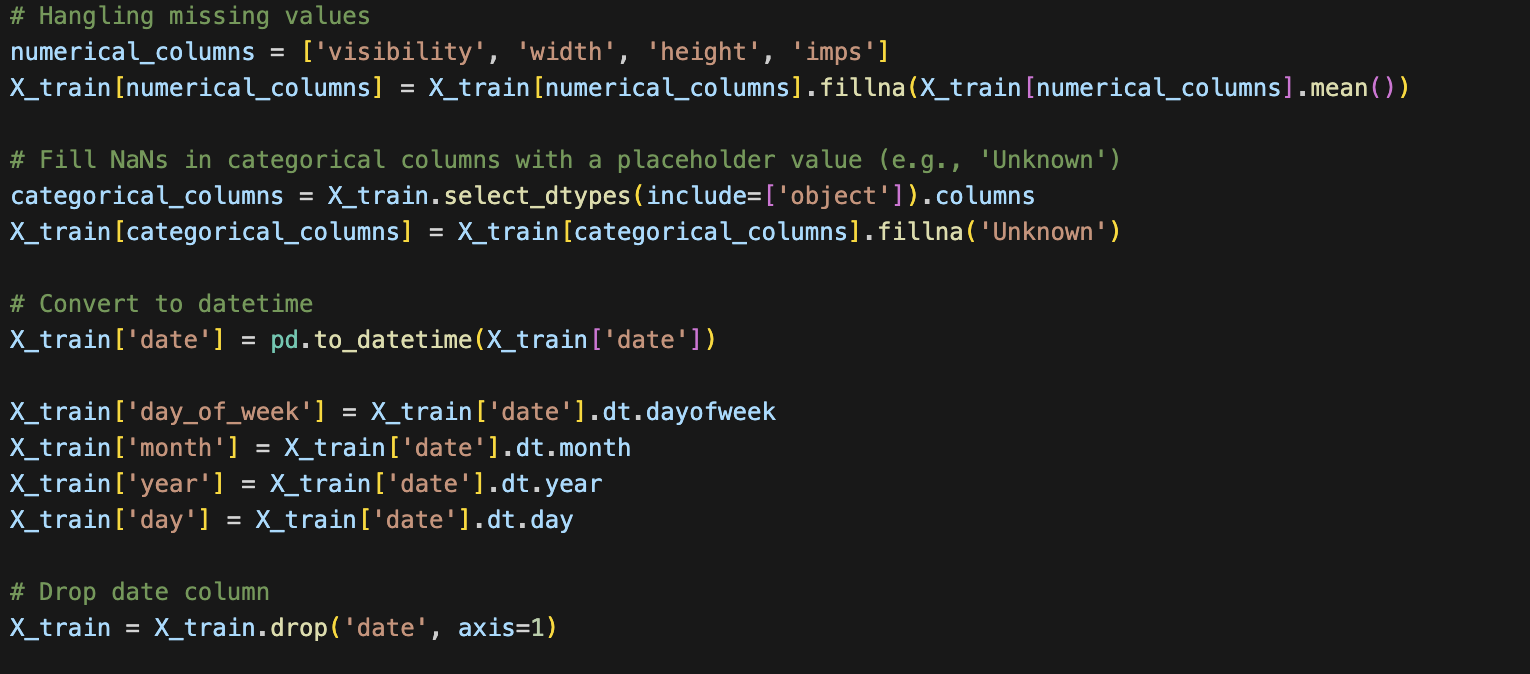
\includegraphics[width=0.8\linewidth]{images/missing_values.png}
	% 	\caption{Handle missing values in the dataset}
	% \end{figure}	
	\begin{block}{Feature scaling and encoding}
		\begin{itemize}
			\item Label encoding for categorical columns
			\item Standardize numerical columns
		\end{itemize}
	\end{block}
\end{frame}


\section{Model}
\begin{frame}{Brain stroming}
	\begin{block}{How to predict click-through rate?}
		\begin{itemize}
			\item Predict the click number using regression model and then calculate the CTR by dividing the predicted click number by the number of impressions
			\item \textbf{Tree-based model} : capture non-linear relationship
			\item \textbf{Deep learning model} : learn complex patterns in the data
		\end{itemize}
		
	\end{block}
	
\end{frame}

\begin{frame}{Model selection}
	\begin{block}{Model selection}
		\begin{itemize}
			\item \textbf{MLP} : Multi-layer Perceptron \XSolidBrush
			\item \textbf{DCN} : Deep \& Cross Network $\checkmark$
		\end{itemize}
	\end{block}
	\begin{block}{Evaluation metric}
		\begin{equation}
			-\frac{\sum_{i}{\text{clicks}_i \times \ln(\hat{y}_i) + (\text{imps}_i - \text{clicks}_i) \times \ln(1 - \hat{y}_i)}}{\sum_{i}{\text{imps}_i}}
		\end{equation}
		\begin{itemize}
			\item \textbf{clicks} : number of clicks
			\item \textbf{imps} : number of impressions
			\item $\hat{y}$ : predicted click-through rate
			\item \textbf{BCE loss : binary cross-entropy loss}
		\end{itemize}
	\end{block}

\end{frame}

\begin{frame}{Model Description}
	\begin{block}{Deep \& Cross Network}
		
		\begin{itemize}
			\item Learn tabular data by transforming categorical features into dense vectors through embeddings
			\item \textbf{Cross Network} : capture the relationship between features with a series of cross layers 
			\item \textbf{Deep Network} : fully connected layers
		\end{itemize}
	\end{block}
	
\end{frame}
\begin{frame}{Model Description}
	\begin{figure}
		\centering
		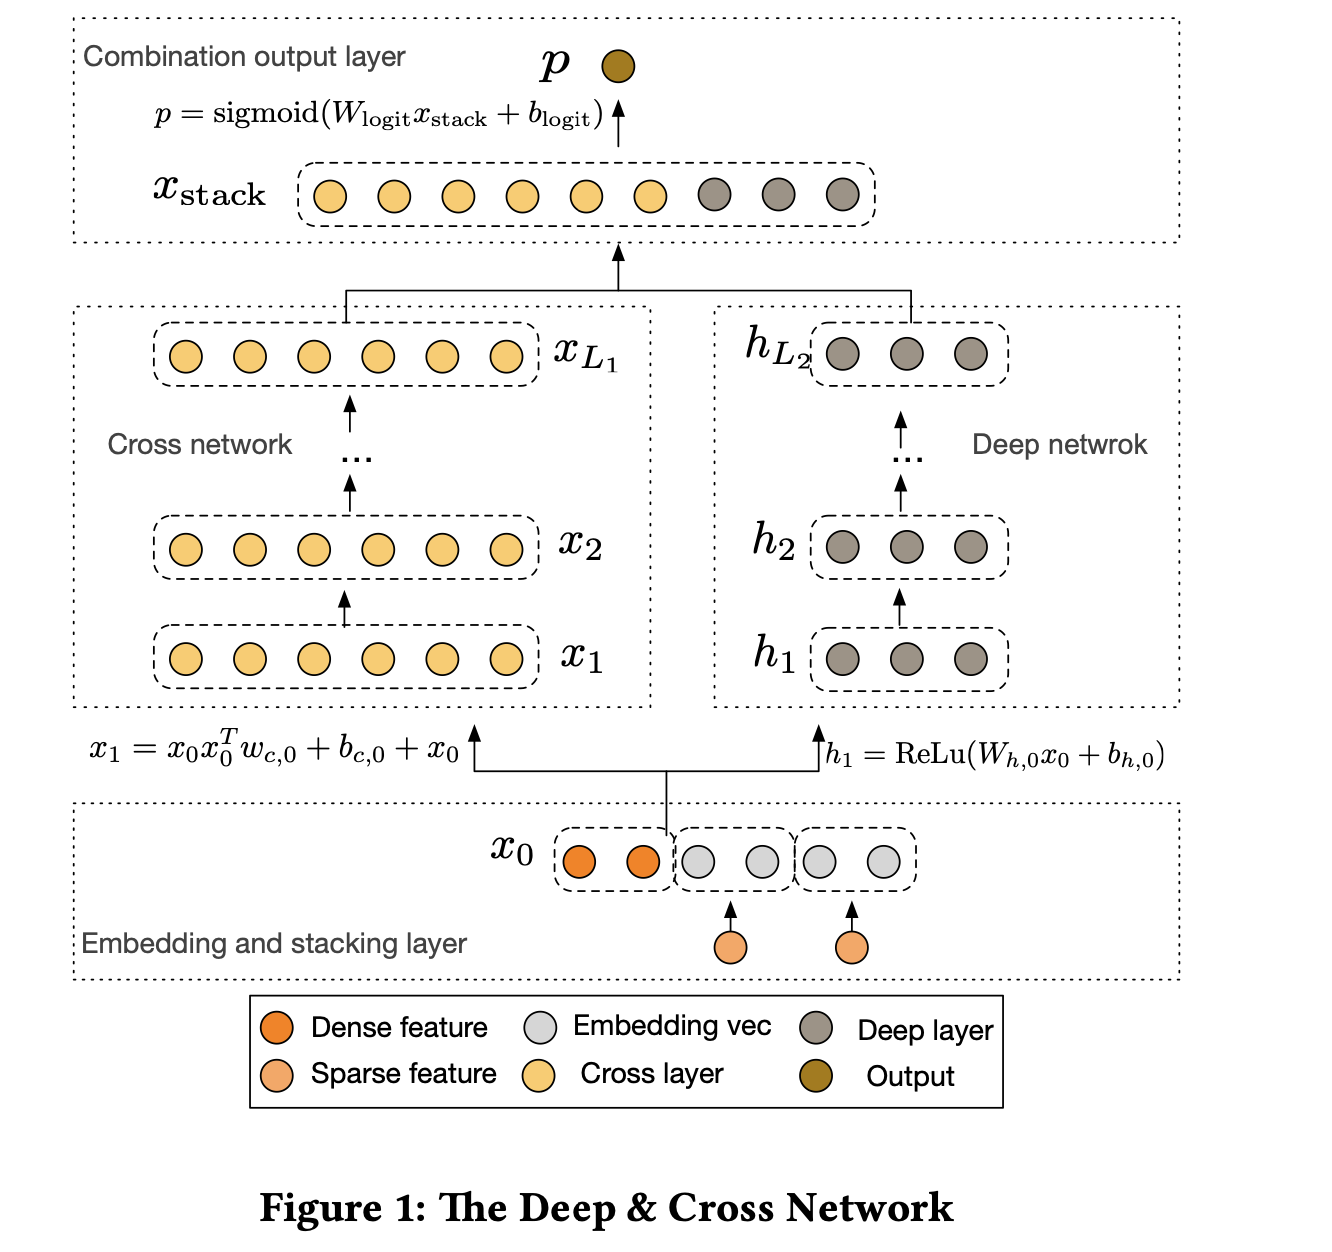
\includegraphics[width=0.8\linewidth]{images/DCN_architecture.png}
		\caption{Deep \& Cross Network}
	\end{figure}
	
\end{frame}

\begin{frame}{Model trainning}
	\begin{block}{Model trainning}
		\begin{itemize}
			\item \textbf{Optimizer} : Adam
			\item \textbf{Learning rate} : 0.001
			\item \textbf{Batch size} : 128
			\item \textbf{Epochs} : 5 or 3
		\end{itemize}
	\end{block}

	
\end{frame}



\section{Results}
\begin{frame}{Results}
	cf. Notbook and .csv
\end{frame}

\begin{frame}{Results}
	\begin{block}{Ratio of non zero ctr}
		\begin{itemize}
			\item BCE CTR label : 1676703 / 2019086
			\item BCE CTR click label :  1439133/ 2019086
			\item MSE CTR label :  319 / 2019086
			\item Clic predict CTR : 1105119/ 2019086
		\end{itemize}
	\end{block}

	\begin{block}{Evaluation metric}
		\begin{itemize}
			\item BCE CTR label : 0.05838478356599808
			\item BCE CTR click label :  0.08586359024047852
			\item MSE CTR label : 0.09446008503437042
			\item Clic predict CTR :  0.4865149259567261
		\end{itemize}
	\end{block}
	
	
\end{frame}

\section{Conclusion}
		

\section{Thank you for your attention!}

\end{document}

